\section{需求分析}
	本次实验需要设计一个程序,程序实现了计算一个有向无环图中最远的两点的距离,
	并且,本程序会打印其中一对的路径。

	
	输入样例:\\
	6 8 \\
	0 1 3 \\
	0 2 1 \\
	0 3 2 \\
	1 4 4 \\
	2 4 7 \\
	3 1 1 \\
	3 5 5 \\
	5 4 6 \\

	输出样例:\\
	The longest disatance is: 13\\
	The longest\_path is:\\
	0 >> 3 >> 5 >> 4 >> end\\


	
\section{概要设计}
	由于我们输入的图为有向无环图G,所以G中会存在一组源点和汇点,则最远两点的距离必定是从源点到汇点的距离。
	所以我们采用了动态规划的思想,即维护一个dis,表示一个顶点最远源点的距离,我们对G进行拓扑排序,按照拓扑排序的顺序对dis更新。
	并且维护每个顶点的father,表示其dis的前驱顶点,方便输出路径,所以我们的数据结构如下


	邻接链表:
	\begin{enumerate}
		\item weight 边权
		\item self 目标顶点
		\item adjvex 当前顶点
		\item next 下一条边
	\end{enumerate}


	结点结构:
	\begin{enumerate}
		\item data 顶点保存的数据
		\item indegree 入度
		\item longest 到 m 顶点的最长距离
		\item father 最长距离路径上的父亲节点
		\item firstAdj 顶点的第一条边
	\end{enumerate}


	图类:
	\begin{enumerate}
		\item vertex 顶点列表,用vector存储
		\item ver\_num 顶点的个数
		\item edge\_num 边的个数
	\end{enumerate}

\section{详细设计}

\begin{algorithm}[htb] 
	\caption{ longest\_path } 
	\label{alg:Framwork} 
	\begin{algorithmic}[1]
		\State 初始化队列topo\_node
		\State 将所有入度为0的结点加入到topo\_node中
		\While{topo\_node不为空}
			\State 从topo\_node中取出front()保存在temp中并弹出
			\For{从temp出发的所有边e}
				\State 将e的终点的顶点入度减1
				\If{e的终点的入度为0}
					\State 将e的终点加入到topo\_node中
				\EndIf
				\If{temp的longest + e->weight > e的终点的longest}
					\State e的终点的longest = temp的longest + e->weight
					\State 更新e的终点的father为temp
				\EndIf
			\EndFor
		\EndWhile
	\end{algorithmic} 
\end{algorithm}

\newpage

\begin{algorithm}[htb] 
	\caption{ create\_graph } 
	\label{alg:Framwork} 
	\begin{algorithmic}[1]
		\State 输入n、m表示顶点的个数和边的个数
		\State 初始化n个顶点
		\For{对于m条边}
			\State 输入x, y, w表示起点,终点,边权
			\State 利用x,y,w初始化边
			\State 将边插入到邻接表中
		\EndFor
	\end{algorithmic} 
\end{algorithm}
\newpage

\section{调试分析报告}
在我们设计的算法中,每个点仅能进入一次队列,且每个边只能被删除一次,所以算法复杂度只和边与点的个数有关。\\
所以算法复杂度为$O(n + e)$

\section{用户使用说明}

用户可以使用IDE或者手动编译源代码main.cpp,获得可执行文件。

笔者使用的gcc版本为8.1.0\\
在使用时,用户需要先输入两个数字n,m表示顶点数与边数,
再依次输入每一条边的具体数值\\
得到的结果中包括最长距离与一条表示最长距离的路径
\section{测试结果}

我们使用的测试样例如下图所示
\begin{figure}[H]
	\centering
	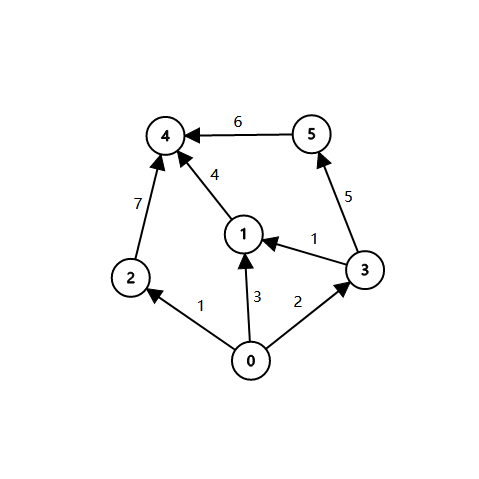
\includegraphics[width=0.5\textwidth]{images/graph.png}
	\caption{graph}
\end{figure}

输入为
6 8 \\
0 1 3 \\
0 2 1 \\
0 3 2 \\
1 4 4 \\
2 4 7 \\
3 1 1 \\
3 5 5 \\
5 4 6 \\


结果为
\begin{figure}[H]
	\centering
	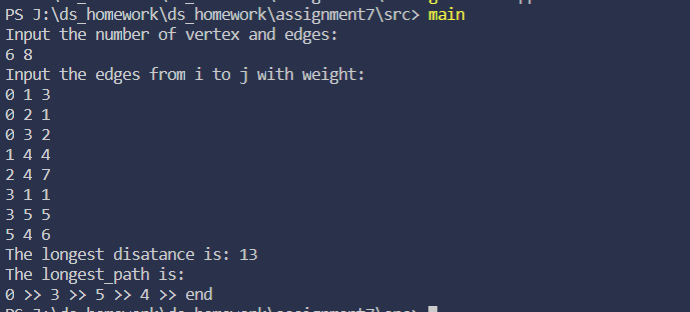
\includegraphics[width=0.5\textwidth]{images/example.png}
	\caption{测试结果}
\end{figure}
